\documentclass{article}
\usepackage[utf8]{inputenc}
\usepackage[margin=1in,includefooter]{geometry}
\usepackage{graphicx}
\usepackage{float}

\begin{document}

\begin{titlepage}
    \begin{center}
    \line(1,0){300} \\
    [0.2in]
    \huge{\bfseries MST Algorithm\\ Comparison Report} \\
    \line(1,0){300} \\
    [1.5cm]
    \textsc{\LARGE Kruskal's vs. Prim's}\\
    [15cm]
    \end{center}
    \begin{flushright}
    \textsc{\large Samy Masadi\\
    CSCI 423\\
    April 26, 2019}
    \end{flushright}
\end{titlepage}

\tableofcontents
\thispagestyle{empty}
\cleardoublepage

\setcounter{page}{1}

\section{Summary}
\hspace{\parindent}The Bubbla Company will be interested to know that both Kruskal's and Prim's algorithms found the same minimum spanning tree for the provided city circuit. As for which performed best, Kruskal's algorithm proved nearly three times faster than Prim's for finding the MST from the city circuit. On the test machine, Kruskal's finished in 0.058 seconds, while Prim's finished in 0.145 seconds.

Although both algorithms have the same time complexity of O(ElogV), for a small graph like the city circuit, time constants in the form of processing or memory access overhead become the determining factor. The most likely culprit for Prim's slightly slower processing may come down to its use of an adjacency list. In the Python code implementation, the adjacency list is represented by a three-dimensional array: verticles in one dimension, the degree of edges in the second dimension, and connected vertices and edge weights in the third. Kruskal's algorithm, meanwhile, only requires a two-dimensional array to represent the graph's edges: edges in the first dimension and edge details in the second. In short, the access times to the arrays, along with other inherent particularities of each implementation, meant Kruskal's worked faster.

In some cases, Kruskal's may find a different MST than Prim's, but for the city circuit the MSTs were the same. The order of edges found was the only difference between them. The MST consists of the following edges: 4-8, 8-9, 3-7, 6-10, 4-5, 9-10, 1-4, 3-4, and 1-2.

As a recommendation for the city circuit problem and other relatively small graphs like it, Kruskal's will serve best, even if only by a fraction of a second. For larger graphs, either algorithm should be suitable as they have the same time complexity.

\newpage
\section{Pseudocode}
Note: The final code implementation for Kruskal's and Prim's algorithms in Python was sourced from GeeksforGeeks. The code for Kruskal's was contributed to GeeksforGeeks by Neelan Yadav [1]. The code for Prim's was contributed by Divyanshu Mehta [2].
\subsection{Kruskal's Algorithm}
\hspace{\parindent}Kruskal(edges):

\hspace{\parindent}sort edges using min heap sort

\hspace{\parindent}for edge in edges:

\hspace{\parindent}\hspace{\parindent}if adding edge does not create a cycle:

\hspace{\parindent}\hspace{\parindent}\hspace{\parindent}result.append(edge)

\hspace{\parindent}\hspace{\parindent}\hspace{\parindent}union(edge)

\hspace{\parindent}print(result)

\subsection{Prim's Algorithm}
\hspace{\parindent}Prim(graph):

\hspace{\parindent}for each vertex:

\hspace{\parindent}\hspace{\parindent}init key value to INF

\hspace{\parindent}\hspace{\parindent}add vertex key value to min heap

\hspace{\parindent}set first vertex key value to 0 to ensure it is selected first

\hspace{\parindent}while min heap is not empty:

\hspace{\parindent}\hspace{\parindent}extract next vertex from min heap

\hspace{\parindent}\hspace{\parindent}after first vertex, start printing edges

\hspace{\parindent}\hspace{\parindent}for each connected vertex:

\hspace{\parindent}\hspace{\parindent}\hspace{\parindent}update key values (weights) in min heap

\newpage
\section{Complexity Analysis}

\subsection{Time Efficiency}
\subsubsection[Kruskal's Algorithm]{Kruskal's Algorithm: O(ElogV)}
Kruskal's algorithm searches vertices for union of edges, which takes logV time. It must do this for each of the edges E it processes.
\subsubsection[Prim's Algorithm]{Prim's Algorithm: O(ElogV)}
The Prim's algorithm implementation utilizes an adjacency list to represent the graph. Accessing all edges in the adjacency list takes E+V time. It must access edges for each of the vertices, where processing a vertex takes logV time. Thus their combination scales with ElogV.

\subsection{Space Efficiency}
\subsubsection[Kruskal's Algorithm]{Kruskal's Algorithm: O(E)}
Kruskal's algorithm focuses on the edges. Since the implementation sorts the edges in a min heap, the overhead scales with the number of edges E.
\subsubsection[Prim's Algorithm]{Prim's Algorithm: O(V)}
The Prim's algorithm implementation places key values of vertices in a min heap, which means the space overhead should scale with the number of vertices V.

\newpage
\section{Screenshot Showcase}
\begin{figure}[H]
    \centering
    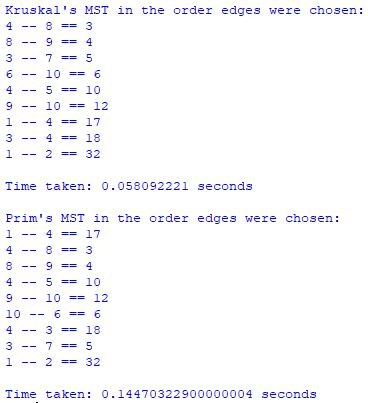
\includegraphics{mst.JPG}
    \caption{Program Results for City Circuit}
\end{figure}

\newpage
\section{References}
[1] Aashish Barnwal. 2019. Kruskal’s Minimum Spanning Tree Algorithm. (2019). Retrieved 26 Apr 2019. https://www.geeksforgeeks.org/kruskals-minimum-spanning-tree-algorithm-greedy-algo-2/ \\ \\
$[2]$ Aashish Barnwal. 2019. Prim’s MST for Adjacency List Representation. (2019). Retrieved 26 Apr 2019. https://www.geeksforgeeks.org/prims-mst-for-adjacency-list-representation-greedy-algo-6/

\end{document}
